\documentclass[12pt, a4paper, oneside, openany, dvipsnames, hidelinks]{book}

  % Enables the use of colour. 
  \usepackage{xcolor}
  % Syntax high-lighting for code. Requires Python's pygments.
  \usepackage{minted}
  % Enables the use of umlauts and other accents.
  \usepackage[utf8]{inputenc}
  % Diagrams.
  \usepackage{tikz}
  % Settings for captions, such as sideways captions.
  \usepackage{caption}
  % Symbols for units, like degrees and ohms.
  \usepackage{gensymb}
  % Latin modern fonts - better looking than the defaults.
  \usepackage{lmodern}
  % Allows for columns spanning multiple rows in tables.
  \usepackage{multirow}
  % Better looking tables, including nicer borders.
  \usepackage{booktabs}
  % More math symbols.
  \usepackage{amssymb}
  % More math fonts, like mathbb.
  \usepackage{amsfonts}
  % More math layouts, equation arrays, etc.
  \usepackage{amsmath}
  % More theorem environments.
  \usepackage{amsthm}
  % More column formats for tables.
  \usepackage{array}
  % Adjust the sizes of box environments.
  \usepackage{adjustbox}
  % Better looking single quotes in verbatim and minted environments.
  \usepackage{upquote}
  % Better blank space decisions.
  \usepackage{xspace}
  % Better looking tikz trees.
  \usepackage{forest}
  % URLs.
  \usepackage{hyperref}
  % For plotting.
  \usepackage{pgfplots}
  % For filler.
  \usepackage{lipsum}
  
  % Various tikz libraries.
  % For drawing mind maps.
  \usetikzlibrary{mindmap}
  % For adding shadows.
  \usetikzlibrary{shadows}
  % Extra arrows tips.
  \usetikzlibrary{arrows.meta}
  % Old arrows.
  \usetikzlibrary{arrows}
  % Automata.
  \usetikzlibrary{automata}
  % For more positioning options.
  \usetikzlibrary{positioning}
  % Creating chains of nodes on a line.
  \usetikzlibrary{chains}
  % Fitting node to contain set of coordinates.
  \usetikzlibrary{fit}
  % Extra shapes for drawing.
  \usetikzlibrary{shapes}
  % For markings on paths.
  \usetikzlibrary{decorations.markings}
  % For advanced calculations.
  \usetikzlibrary{calc}
  
  % GMIT colours.
  \definecolor{gmitblue}{RGB}{20,134,225}
  \definecolor{gmitred}{RGB}{220,20,60}
  \definecolor{gmitgrey}{RGB}{67,67,67}
  
  % Tell minted to use the following colour scheme. 
  \usemintedstyle{manni}
  
  %% Change these:
  \newcommand{\thesistitle}{The Art of Computer Programming -- A difficult book to understand}
  \newcommand{\thesisauthor}{Ian McLoughlin}
  \newcommand{\thesisadvisor}{Dr Ian McLoughlin \\[1mm] Dr Ian McLoughlin \\[1mm] Dr Ian McLoughlin}
  \newcommand{\thesisdegree}{Master of Science}
  \newcommand{\thesisdate}{\today}
  \newcommand{\thesisinstitute}{Galway-Mayo Institute of Technology}
  \newcommand{\thesisdepartment}{Department of Computer Science and Applied Physics}
  %% End of things to change.

  % Begin the document.  
  \begin{document}
    % Include the titlepage  
    
%% Change these:
\newcommand{\thesistitle}{My Excellent PhD Thesis on the Topic of Cool Stuff I Wrote About}
\newcommand{\thesisauthor}{by Ian McLoughlin}
\newcommand{\thesisadvisor}{Advisors:\\Dr Ian McLoughlin, Dr Ian McLoughlin, and Dr Ian McLoughlin}
\newcommand{\thesistype}{PhD Thesis}
\newcommand{\thesisdate}{Submitted: \today}
\newcommand{\thesisdepartment}{Department of Computer Science and Applied Physics}
\newcommand{\thesisfunding}{This Research has been supported by the Atlantic Technological University under the Postgraduate Research Training Programme in Modelling and Computation for Health and Society (MOCHAS PRTP).}
%% End of things to change.

% The title page.
\begin{titlingpage}
  
  {\noindent\Huge\textbf{\thesistitle}\par}
  \vspace{12mm}
  {\noindent\LARGE\textbf{\thesisauthor}\par}
  \vspace{26mm}
  {\noindent\Large\textbf{\thesistype}\par}
  \vspace{2mm}
  {\noindent\Large\thesisdepartment\par}
  \vspace{2mm}
  {\noindent\Large\thesisadvisor\par}
  \vspace{2mm}
  {\noindent\Large\thesisdate\par}
  \vspace{26mm}
  {\noindent\thesisfunding\par}


  \AddToHookNext{shipout/background}{
    \begin{tikzpicture}[remember picture, overlay, inner sep=0pt, outer sep=0pt]
    \node[anchor=south east] at ([xshift=-32mm,yshift=12mm]current page.south east) {
      \includegraphics[width=6cm]{img/atu_logo.png}
    };
    \end{tikzpicture}
  }
  
\end{titlingpage}
    
    % Set the correct page number.
    \setcounter{page}{2}

    % Insert the table of contents.
    \tableofcontents

    % Include the chapter.
    %!TEX root = ../thesis.tex

\chapter*{Abstract}


Writing a compelling abstract for a Ph.D. thesis requires conciseness, clarity, and the ability to convey the significance of your research. Here are some tips to help you craft an effective abstract.
(1) Clearly State the Problem:
Begin by clearly stating the problem or question your research addresses.
Be concise and specific about the problem you are investigating.
(2) Highlight the Objective:
Clearly state the main objective of your research.
What are you contributing to the field of study?
Make it evident how your work fits into the broader context.
(3) Provide a Brief Overview of Methods:
Mention the key methods used in your research.
Briefly explain the tools or frameworks you used to address the problem.
However, avoid going into excessive detail.
(4) Present Key Results:
Summarize the main findings and results of your research. 
Highlight any breakthroughs, novel insights, or contributions your work has made to the field.
(5) Contextualize the Significance:
Communicate the significance and relevance of your research. 
Explain how your findings contribute to and address gaps in the field.
(6) Use Concise and Accessible Language:
Write in a clear, concise, and accessible language.
Avoid unnecessary jargon that may be unclear to readers outside your specific subfield of study.
Remember that the abstract serves as a short summary of your entire Ph.D. thesis.
It provides readers with a quick overview of your research. Striking the right balance between conciseness and informativeness is key.
Put your best foot forward without overstating your findings.




\chapter*{About the Author}
When writing about yourself, highlight your academic background, research interests, accomplishments, and any relevant experiences.
Here are some tips to help you craft an effective blurb.
(1) Start with a Strong Opening:
Begin with a concise and engaging statement that captures the reader's attention. For example, you might start with a brief description of your academic journey or research focus.
(2) Highlight Your Academic Background:
Provide a brief overview of your academic qualifications, including your degree(s) and any relevant academic honors or awards you have received.
(3) Emphasize Your Research Interests:
Clearly articulate your research interests and the topics you are passionate about. Briefly mention any specific areas of mathematics or related fields that you have focused on in your thesis work.
(4) Showcase Your Accomplishments:
Highlight any significant achievements or contributions you have made in your field. This could include publications, conference presentations, research projects, or collaborations.
(5) Include Relevant Experiences:
Mention any relevant academic or professional experiences that have shaped your research interests and expertise. This could include internships, research assistantships, teaching positions, or involvement in academic societies.
    \chapter{Introduction}
This chapter should introduce the thesis.
Provide a context for the research, and explain the layout of the chapters.
Make sure you use references~\cite{einstein}.

\section{Context}

\lipsum[1-4]

\section{Layout}

\lipsum[1-4]
    \chapter{Literature review}
This chapter should give a comprehensive overview of the relevant literature.
Again, make sure you use referncing throughout.


\section{Methodology}
\lipsum[5-15]

\section{Literature}
\lipsum[16-25]

    \chapter{Methodology}

You are expected to be methodical in your work, so that it could and can be
reproduced and replicated by others to verify your results.
If you are clear in your methodology, you will have a better chance of someone
building on your work \cite{villaneuva18}.
That will lead to more people being interested in what you have done, and will
give you a higher profile.
Remember that undergraduate students will sometimes do projects based on
academic research, so it's a good idea to be explicit enough that they can
easily replicate your results.

It is important that you demonstrate that you were methodical from the start.
While it is tempting to play around with various algorithms or techniques
before you really sit down to work.
If you take five minutes beforehand to think through what you are about to do
and write it down, you will quickly build up a portfolio of writing and results
that can go into your thesis.
There is often very little pracitcal difference between being methodical and
playing around -- it's largely in your attitude while you are doing the work.

Note that \LaTeX has a lot of nice functionality for creating various types of
plots and diagrams.
Check out the nice graphs in Figure \ref{tikz:graphs}.

\lipsum[26]

\begin{figure}[ht]
  \centering
  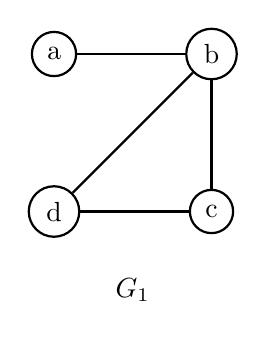
\begin{tikzpicture}
    \begin{scope}[every node/.style={circle,thick,draw}]
      \node (a) at (0,2) {a};
      \node (b) at (2,2) {b};
      \node (c) at (2,0) {c};
      \node (d) at (0,0) {d};
    \end{scope}
    \begin{scope}[every edge/.style={draw=black,thick}]
      \path (a) edge (b);
      \path (b) edge (c);
      \path (b) edge (d);
      \path (c) edge (d);
    \end{scope}
    \node () at (1,-1) {$G_1$};
  \end{tikzpicture}
  \hspace{1.5cm}
  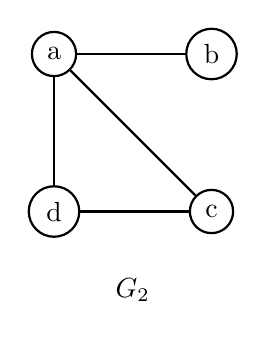
\begin{tikzpicture}
    \begin{scope}[every node/.style={circle,thick,draw}]
      \node (1) at (0,2) {a};
      \node (2) at (2,2) {b};
      \node (3) at (2,0) {c};
      \node (4) at (0,0) {d};
    \end{scope}
    \begin{scope}[every edge/.style={draw=black,thick}]
      \path (1) edge (2);
      \path (1) edge (3);
      \path (1) edge (4);
      \path (3) edge (4);
    \end{scope}
    \node () at (1,-1) {$G_2$};
  \end{tikzpicture}
  \caption{Nice pictures}
  \label{tikz:graphs}
\end{figure}

\section{Vector Spaces}

A \textbf{vector space} $V$ over a field $\mathbb{F}$ is a set equipped with two operations:

\begin{itemize}
    \item Vector addition: $+: V \times V \rightarrow V$, denoted as $(\mathbf{v}, \mathbf{w}) \mapsto \mathbf{v} + \mathbf{w}$.
    \item Scalar multiplication: $\cdot: \mathbb{F} \times V \rightarrow V$, denoted as $(\lambda, \mathbf{v}) \mapsto \lambda \mathbf{v}$.
\end{itemize}
These operations must satisfy the following properties for all $\mathbf{u}, \mathbf{v}, \mathbf{w} \in V$ and $\lambda, \mu \in \mathbb{F}$:

\begin{enumerate}
    \item \textbf{Addition is commutative}: $\mathbf{u} + \mathbf{v} = \mathbf{v} + \mathbf{u}$.
    \item \textbf{Addition is associative}: $(\mathbf{u} + \mathbf{v}) + \mathbf{w} = \mathbf{u} + (\mathbf{v} + \mathbf{w})$.
    \item \textbf{Additive identity}: There exists a vector $\mathbf{0} \in V$ such that $\mathbf{v} + \mathbf{0} = \mathbf{v}$ for all $\mathbf{v} \in V$.
    \item \textbf{Additive inverse}: For every vector $\mathbf{v} \in V$, there exists a vector $-\mathbf{v} \in V$ such that $\mathbf{v} + (-\mathbf{v}) = \mathbf{0}$.
    \item \textbf{Scalar multiplication is distributive over vector addition}: $\lambda (\mathbf{v} + \mathbf{w}) = \lambda \mathbf{v} + \lambda \mathbf{w}$.
    \item \textbf{Scalar multiplication is distributive over scalar addition}: $(\lambda + \mu) \mathbf{v} = \lambda \mathbf{v} + \mu \mathbf{v}$.
    \item \textbf{Scalar multiplication is associative}: $(\lambda \mu) \mathbf{v} = \lambda (\mu \mathbf{v})$.
    \item \textbf{Scalar multiplication identity}: $1 \cdot \mathbf{v} = \mathbf{v}$, where $1$ is the multiplicative identity in $\mathbb{F}$.
\end{enumerate}


\section{Dirac Notation}
Dirac notation, also known as bra-ket notation, is a powerful and concise mathematical notation used extensively in quantum mechanics.
It was introduced by the physicist Paul Dirac and provides a convenient way to represent vectors, linear operators, and inner products in quantum mechanics.
Here's a breakdown of the components of Dirac notation:

\begin{description}
  \item[Ket notation $\ket{\psi}$:]
  A ket is represented by a column vector enclosed within vertical bars.
  It represents a state vector in a complex vector space.
  For example, $\ket{\psi}$ could represent the state of a quantum system.

  \item[Bra notation $\bra{\psi}$:]
  A bra is represented by a row vector enclosed within angular brackets.
  It represents the complex conjugate transpose of a ket vector.
  If $\ket{\psi}$ represents a state vector, then $\ket{\psi}$ represents the corresponding bra vector.

  \item[Inner product ($\braket{\psi \mid \psi}$):]
  The inner product of two vectors is represented by placing a bra vector on the left and a ket vector on the right, enclosed within angular brackets.
  It yields a complex number and is a measure of the "overlap" between the two vectors.
  In quantum mechanics, the inner product is used to calculate probabilities and to determine the expectation values of observables.

  \item[Outer product ($\ket{\psi}\bra{\phi}$):]
  The outer product of two vectors is represented by placing a ket vector on the left and a bra vector on the right.
  It results in a linear operator known as a ket-bra or dyad, which maps one vector to another.
  In quantum mechanics, outer products are used to represent quantum operators.

  \item[Operators ($A\ket{\psi}$):]
  If $A$ is a linear operator, its action on a ket vector $\ket{\psi}$ is represented by placing the operator to the left of the ket vector.
  This notation shows the result of applying the operator to the state vector.
\end{description}
Dirac notation offers several advantages:
\begin{description}
    \item[Clarity and Conciseness:]
    It provides a concise representation of complex mathematical objects, making expressions and calculations easier to write and understand.
    \item[Flexibility:]
    It can be easily extended to represent complex operations and concepts in quantum mechanics, such as composite systems, entanglement, and measurement.
    \item[Computational Efficiency:]
    Dirac notation simplifies many calculations in quantum mechanics, such as computing inner products, expectation values, and transition probabilities.
\end{description}
Overall, Dirac notation is a fundamental tool in quantum mechanics, enabling physicists to express and manipulate quantum states and operations in a clear and efficient manner.

    \chapter{Prototype code}


\section{XML}
Here's some nicely formatted XML:
\begin{minted}{xml}
<this>
  <looks lookswhat="good">
    Good
  </looks>
</this>
\end{minted}


    \chapter{More chapter}
Table \ref{table:mytable} is a nice table.

\begin{table}[h]
  \centering
  \begin{tabular}{cc}
    \toprule \\
    Column 1 & Column 2 \\
    \midrule \\
    Hello & world! \\
    \bottomrule
  \end{tabular}
  \caption{A table.}
  \label{table:mytable}
\end{table}


    \chapter{Conclusion}

What Should the Conclusion Section of a PhD Thesis Include?
The conclusion section of a Ph.D. thesis serves as the final chapter where you summarize the key findings of your research, discuss their implications, and reflect on the contributions of your work to the field.
Below are some items you should include in the conclusion.

\subsection{Summary of Key Findings}
Recapitulate the main results and outcomes of your research.
Summarize the key findings, discoveries, or insights obtained through your investigation.
    
    
\subsection{Discussion of Research Questions or Hypotheses}
Reflect on how your research has addressed the research questions or hypotheses posed at the beginning of your study.
Discuss whether your findings support or refute the initial hypotheses and how they contribute to advancing knowledge in the field.
    
    
\subsection{Implications and Contributions}
Discuss the broader implications of your research findings. Explain how your work contributes to theoretical understanding, practical applications, or methodological advancements within your discipline.
Highlight the significance of your research and its potential impact on academic research, policy-making, industry practices, or society as a whole.
    
    
\subsection{Limitations and Future Directions}
Acknowledge any limitations or constraints encountered during your research, such as methodological limitations, data constraints, or external factors beyond your control.
Discuss opportunities for future research that arise from your findings.
Identify unanswered questions, areas for further investigation, or new research directions that could build upon your work.
    
    
\subsection{Reflection and Personal Insights}
Reflect on your journey as a researcher throughout the Ph.D. process.
Discuss any challenges, successes, or unexpected discoveries you encountered along the way.
Share personal insights or lessons learned from conducting your research, including any changes in your perspectives, methodologies, or research practices.
    
    
\subsection{Final Remarks}
Provide a concluding statement that synthesizes the main points of your conclusion.
Emphasize the significance of your research and its broader implications for the field.
Express gratitude to those who have supported you during your Ph.D. journey, including mentors, advisors, colleagues, friends, and family members.

Overall, the conclusion section of a Ph.D. thesis should effectively summarize your research journey, highlight the contributions of your work, and articulate its significance within the broader scholarly context.
It should leave the reader with a clear understanding of the key takeaways from your study and inspire further inquiry and exploration in the field.


    % Include the bibliography with IEEE style.
    \bibliographystyle{ieeetr}
    \bibliography{bibliography}
  \end{document}
